%%%%%%%%%%%%%%%%%%%%%%%%%%%%%%%%%%%%%%%%%%%%%%%%%%%
%
%  New template code for TAMU Theses and Dissertations starting Fall 2012.  
%  For more info about this template or the 
%  TAMU LaTeX User's Group, see http://www.howdy.me/.
%
%  Author: Wendy Lynn Turner 
%	 Version 1.0 
%  Last updated 8/5/2012
%
%%%%%%%%%%%%%%%%%%%%%%%%%%%%%%%%%%%%%%%%%%%%%%%%%%%

%%%%%%%%%%%%%%%%%%%%%%%%%%%%%%%%%%%%%%%%%%%%%%%%%%%%%%%%%%%%%%%%%%%%%%
%%                           SECTION I
%%%%%%%%%%%%%%%%%%%%%%%%%%%%%%%%%%%%%%%%%%%%%%%%%%%%%%%%%%%%%%%%%%%%%


\pagestyle{plain} % No headers, just page numbers
\pagenumbering{arabic} % Arabic numerals
\setcounter{page}{1}


\chapter{\uppercase {Introduction and Background}}

Seismic reflection is the most important method used in the oil \& gas industry. Huge amount of seismic data are already generated and processed for several decades in such area, although there is no such big data concept at that time. In the data processing steps such as acquisition, migration and interpretation, it involves a lot of domain-specfic specialists and computer scientists to cowork together. Since the seismic data processing is both computation- and data-intensive, the High Performance Computing (HPC) technology was widely used in this area; The typical working flow should be: geophysicists use Matlab to verify algorithms on small sample data, then submit verified algorithms to computer scientists who will translate them into MPI codes that could run efficiently with actual data on cluster, which is time-consuming and high-stakes procedure due to the inconsistent results on sample and actual data. With the improvement of the data acquisition methods and requirement of high resolution for advance processing algorithm, the volume size of seismic data increases drastically, which is big challenge for the traditional way. In this paper, we will try to setup a seismic data processing platform on which all stakeholders could work with same data sets and algorithms without much performance expense.

\section{Seismic Data Processing Flow}
As a dominant method of exploration geophysics in oil \& gas area, reflection seismology (or seismic reflection) uses the principles of seismology to estimate the properties of the Earth's subsurface from reflected seismic waves \cite{seisreflection}. Although the theory of reflection is simple, but the processing flow is more compilicate in pratical scenario. The main steps in such work flow include: data acquistion, data processing, data interpretation and attribute analysis.

In the data acquistion stage, seismic sources such as dynamite or air gun are used to generate seismic waves, and the waves are reflected or refracted while encountering different type of materials underground and are recoreded by the receivers. It becames more complicated in non-normal incidence, such as refraction, multiple reflection and cultural noise, and all these factors need to be considered in processing stage. The first step is pre-processing after acquiring the survey data, in which main steps are removing noise and boosting signal leve. Velocity analysis, stacking and migration are main tasks in seismic data processing, and after migration the seismic events are geometrically re-located in either space or time to the location the event occurred in subsurface and create a complete image of subsurface\cite{seisreflection}. The main goal of seismic interpretation is trying to find petroleum reservoir. But such task requires deep analysis of seismic attributes and geophysics related knowledge, and involves huge amount human resource such as computer scientists, geologists and geophysicists etc. In this paper, we focus on latter stage and built a platform that facilitates seismic attributes extraction and analytics.   

\begin{figure}[h]
\centering
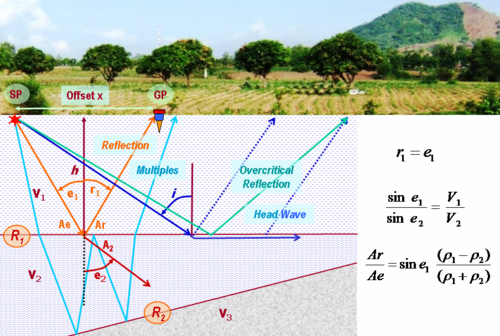
\includegraphics[scale=1]{seismic_reflection_principal.png}
\caption{Seismic Reflection Outlines\cite{seisreflection}}
\label{seismic_reflection}
\end{figure}

%A landscape figure should be shown below. 
%%%%%%%%%%%%%%%%%%%%%%%%%%%%%%%%%%%%%%%%%%%%%%%%%%%%%%
%\begin{sidewaysfigure}[H]
%\centering
%
\includegraphics[scale=.50]{figures/Penguins.jpg}
%\caption{TAMU figure - This is an example of a long figure title with a landscape figure.  Figure titles need to be single-spaced within and double spaced between in the list of figures.}
%\label{fig:tamu-fig1-1}
%\end{sidewaysfigure}
%%%%%%%%%%%%%%%%%%%%%%%%%%%%%%%%%%%%%%%%%%%%%%%%%%%%%%


\section{Current Processing Methodlogy}
HPC technology has been used to process seismic data for several decades. In most current big oil \& gas companines or related service companines, there must have an IT department and a huge group of geophysicists or data scientists forming the research team. In normal case, each small team set up a research project, and then develop new models or algorithms to verify their idea. In this stage, they only use synthetic or historical small data to do experiments, and their programming environment is MATLAB in general. But why did not they experimentalize on big cluster with actual seismic data? The main reason is geophysicists are not familiar with HPC environment, and their main target is to verify the validity of algorithms or models, but not the performance. The volume size of actual data is usually very large and will take much more time to run with MATLAB codes. After research work was finished and got approval, geophysicists will submit their MATLAB codes to IT departments, and then experts in HPC domain will translate such codes into MPI codes or hybrid OpenMP/MPI codes and verify them on high performance cluster with actual seismic data. If there are any problems in this stage, the original authors need to be involved to find the root cause, and the results were either changing the algorithms or models by geophysicists or modification of programming implementation. To make such research project become a mature product, it often will take one more year with several iterations.

%\subsection{This is a Very Long Subsection Title This is a Very Long Subsection Title}


\section{The Big Challeges}
In fact, there are problems in current seismic data analytics flow. As shown in previous section, the MATLAB codes work well on sample data do not mean they could run successfully in parallel after translation into MPI codes. The test cases of MATLAB codes are not enough, and the parallization itself may also procuce new problems. The biggest challege in such area is burst increase of data volume size, which also need more advance algorithm and models to process data. For instance, the volume size of high dimension such as 3D even 4D seismic data and high density seismic data are growing exponentially, so seismic data processing becomes bothe computation- and data- intensive problem.  The traditional HPC programming model is good at handle computation intense case, but with the huge increase of volume size, data movement between nodes is the big bottleneck even with infiniband connections. Another problem is the maintainence and reuse of legacy codes; Most of HPC codes in such area were written in Fortran to achieve high performance, the readability and maintenance of such program are also challeges for beginners. With the improvement of CPU computation power and programming architecture, it should not only focus on executation time, but also the overall perfromance of whole team. 

